\chapter{METODE PENELITIAN}

Bab ini memaparkan tentang metodologi penelitian yang digunakan pada penelitian ini yaitu tahap analisis penyelesaian masalah dan implementasi.

\section{Desain dan analisis penyelesaian masalah}

Pada permasalahan pencarian Ulam non interaktif, penjawab tidak diperbolehkan menjawab sebelum penanya selesai menanyakan seluruh query. Ada dua pendekatan berbeda yang dapat dilakukan untuk menyelesaikan masalah tersebut, yaitu menggunakan repetisi pencarian biner dan menggunakan kode biner. Perlu diketahui bahwa kedua solusi tersebut tidak saling berhubungan.

\subsection{Solusi menggunakan kode biner}

Kita tahu bahwa permasalahan Ulam dengan ruang pencarian $M$ dan maksimal bohong $e$ dapat deselesaikan dengan membuat $q$ query yang jika ditranspose akan membentuk kode biner $(n,M,d)_2$ dimana $d = 2*e+1$. Oleh karena itu tahap selanjutnya adalah jika diketahui $M$ dan $d$, bagaimana membuat seminimal mungkin $n$ agar kode biner $(n,M,d)_2$ valid. Langkah utama untuk membuat kode biner tersebut dengan $M$ dan $e$ yang diketahui adalah dengan menambahkan kode secara iteratif agar minimal jarak Hamming kode biner mencapai $e$.

Gambar \ref{fig:hamming1} menunjukkan ilustrasi jika $M = 8$, $n = 3$, dan $d = 1$. Tabel pada gambar  menunjukkan jarak Hamming antar codeword $x$ dan $y$, sehingga dapat disimpulkan jarak Hamming minimal adalah 1. Gambar \ref{fig:hamming2} adalah penambahan dua kode dari Gambar \ref{fig:hamming1} sehingga $n = 5$ dan $d = 2$.

\begin{figure}
\centering
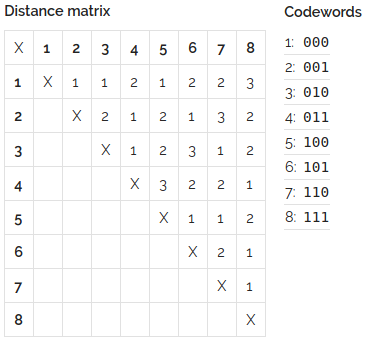
\includegraphics[scale=0.7]{../img/hamming1.png}
\caption{Hasil tabel jarak Hamming pada $(3,8,1)_2$}
\label{fig:hamming1}
\end{figure}

Diagram alir algoritma untuk menyelesaikan permasalahan Ulam non interaktif ada pada Gambar \ref{fig:flow_binarycode}. Setelah dilakukan input ruang pencarian $M$ dan maksimal bohong $e$, simpan $M$ untuk digunakan pada saat output query terakhir. Ubah $M$ menjadi perpangkatan dua terdekat, karena algoritma selanjutnya hanya dapat berjalan jika $M$ adalah perpangkatan dua. Pada subbab selanjutnya akan dijelaskan algoritma untuk menggunakan query generator dan juga algoritma utama untuk menyelesaikan permasalahan Ulam non interaktif.

\begin{figure}
\centering
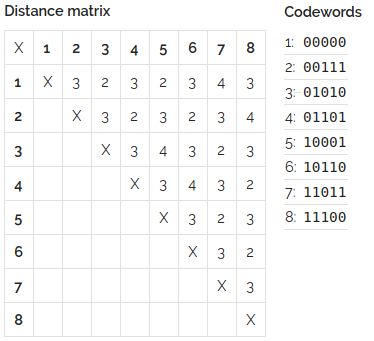
\includegraphics[scale=0.7]{../img/hamming2.png}
\caption{Hasil tabel jarak Hamming pada $(5,8,2)_2$}
\label{fig:hamming2}
\end{figure}

Proses pencarian mendalam (\textit{exhaustive search}) menggunakan pendekatan \textit{greedy} akan dilakukan sebagai pra proses dan hasil pra proses tersebut akan langsung dimasukkan ke dalam kode sumber solusi, karena proses pencarian mendalam memiliki kompleksitas $O(M^3)$ sedangkan jika dilakukan sebagai pra proses dan dimasukkan langsung ke dalam kode sumber solusi sebagai array akan mengurangi kompleksitas menjadi $O(1)$. Namun untuk keperluan pengujian, algoritma kode biner tanpa tabel pencarian (algoritma kode biner yang melakukan proses pencarian mendalam) akan dibandingkan dengan algoritma kode biner dengan tabel pencarian (proses pencarian mendalam dilakukan sebagai pra proses).

\begin{figure}
\centering
\begin{tikzpicture}[node distance=2cm,on grid,auto]
% nodes
\node (n0) [start] {Start};
\node (n1) [io,below of=n0] {Input $M$, $e$};
\node (n2) [process,below of=n1,align=center] {$real\_M = M$\\$m$ = ceil($\log_2(M)$)\\$M=2^m$};
\node (n3) [process,below of=n2,align=center] {$code$ = Generate all possible query using query generator};
\node (n4) [process,below of=n3,align=center] {$code\_order$ = Preloaded exhaustive search($2 \leq 2^m  \leq 4096$, 16)};
\node (n5) [process,below of=n4] {$minimal$ = Generate minimal query};
\node (n6) [process,below of=n5] {$queries$ = Generate actual query};
\node (n7) [io,below of=n6] {Print all the $queries$};
\node (n8) [start,below of=n7] {End};
% arrows
\draw[arrow] (n0) -- (n1);
\draw[arrow] (n1) -- (n2);
\draw[arrow] (n2) -- (n3);
\draw[arrow] (n3) -- (n4);
\draw[arrow] (n4) -- (n5);
\draw[arrow] (n5) -- (n6);
\draw[arrow] (n6) -- (n7);
\draw[arrow] (n7) -- (n8);
\end{tikzpicture}
\caption{Diagram alir solusi menggunakan pembobotan Berlekamp}
\label{fig:flow_binarycode}
\end{figure}

\subsubsection{Algoritma pembangkitan query}

Untuk membuat kode biner $(n,M,d)_2$, maka diperlukan algoritma untuk membangkitkan kode. Karena setiap satu query adalah hasil transpose dari sebuah kolom pada kode biner, setiap kolom pada kode biner dapat dibuat dari bitstring pembangkit $s = \mathbb{F}_2^m$ yang jika diubah menjadi integer akan memiliki rentang $0 \leq s < M$. Oleh karena itu ada $M-1$ macam $s$ karena $s=0$ akan menghasilkan query $\vec{0}$ yang tidak akan menghasilkan jarak Hamming pada kode biner.

Algoritma untuk membuat sebuah query dengan code generator ditunjukkan pada Kode Sumber \ref{alg:generate_query}. Input dari fungsi ini adalah ruang pencarian $M$ dan bilangan bulat $s$ yang akan diubah menjadi sebuah query. Pertama-tama siapkan bilangan bulat $0 \leq i < M$ untuk perulangan kombinasi linier pada $s$ seperti yang ditunjukkan pada baris \ref{alg:kombinasi_linier_for}. Lalu kalikan semua bit dari $s$ dan $i$ seperti yang ditunjukkan pada baris \ref{alg:kombinasi_linier}. Lalu jumlahkan semua bit hasil perkalian $s \cdot i$ seperti yang ditunjukkan pada baris \ref{alg:counting_bit_set}. Lalu hasil semua kombinasi linear akan ditampung pada string $query$ seperti yang ditunjukkan pada baris \ref{alg:save_query}. Total query akan memiliki panjang $M$.

\begin{algorithm}[h]
\caption{Algoritma membuat sebuah query dengan code generator}
\label{alg:generate_query}
\Fn{generate\_query($M$, $s$)}{
\KwData{$M$ search space, $s$ initial generator number}
\KwResult{$query$}
  $query$ = ""\;
  \For{$i = 0$ \KwTo $M$}{\label{alg:kombinasi_linier_for}
    $bitstring = i\ \&\ s$\;\label{alg:kombinasi_linier}
    $binary = 0$\;
    \While{$bitstring$}{\label{alg:counting_bit_set}
      $binary \mathrel{\wedge}= bitstring\ \&\ 1$\;
      $bitstring \mathrel{>>}= 1$\;
    }
    $query \mathrel{+}= binary$\;\label{alg:save_query}
  }
  \Return $query$\;
}
\end{algorithm}

\begin{figure}
\centering
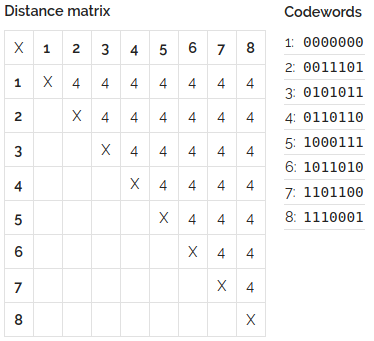
\includegraphics[scale=0.5]{../img/hamming3.png}
\caption{Hasil tabel jarak Hamming pada $M=8$ dan $n=7$}
\label{fig:perfect8}
\end{figure}

\begin{figure}
\centering
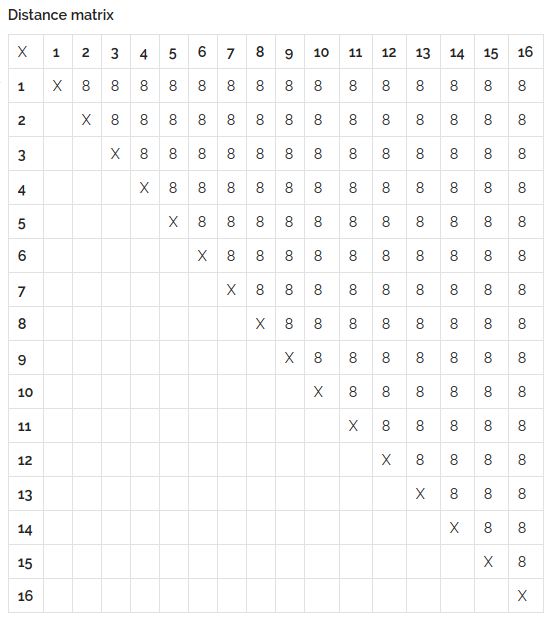
\includegraphics[scale=0.45]{../img/perfect16.png}
\caption{Hasil tabel jarak Hamming pada $M=16$ dan $n=15$}
\label{fig:perfect16}
\end{figure}

Setelah melakukan percobaan menggunakan seluruh $M-1$ query untuk $M$ ruang pencarian, didapatkan seluruh jarak hamming setiap codeword adalah $M/2$. Gambar \ref{fig:perfect8} adalah contoh pada $M=8$ dan $n=7$. Lalu Gambar \ref{fig:perfect16} adalah contoh pada $M=16$ dan $n=15$. Dari hasil tersebut dapat disimpulkan bahwa dengan melakukan seluruh $M-1$ macam query dengan generator untuk ruang pencarian $M$, akan didapatkan kode biner dengan $d=M/2$. Kode biner pada Persamaan \ref{eq:perfectbinarycode} disebut sempurna karena seluruh jarak Hamming pada setiap codeword yang berbeda bernilai $d = M/2$.

\begin{equation}
\label{eq:perfectbinarycode}
\text{Terdapat kode biner sempurna }(M-1, M, M/2)_2
\end{equation}

\begin{align}
q_{rep} &= d\ \backslash\ (M/2) \label{eq:qrep} \\
d_{mod} &= d \text{ mod } (M/2) \label{eq:dmod}
\end{align}

Oleh karena itu jika kita membutuhkan query yang menghasilkan $d = M/2$, maka gunakan seluruh $M-1$ query dengan generator. Sedangkan jika kita membutuhkan query yang menghasilkan $d < M/2$, pilih sesedikit mungkin $n$ query agar menghasilkan $d$ yang dibutuhkan. Dari kebutuhan tersebut, dibuatlah rumus $q_{rep}$ dan $d_{mod}$. Nilai $q_{rep}$ yang didapat dari Persamaan \ref{eq:qrep} adalah jumlah perulangan yang dilakukan terhadap $M-1$ query untuk mencapai solusi. Nilai $d_{mod}$ yang didapat dari Persamaan \ref{eq:dmod} adalah sisa jarak Hamming $d$ yang dibutuhkan untuk mencapai solusi. Cara untuk mencari jumlah query sisa untuk menghasilkan jarak Hamming distance $d_{mod}$ ada pada subbab selanjutnya.

\subsubsection{Pencarian mendalam untuk mendapatkan urutan kode biner}

Algoritma solusi menggunakan generator matrix harus membuat urutan $s$ tertentu sedemikian hingga seminimal mungkin jumlah query $n$ yang dihasilkan dari $\vec{s} = \{s_1, \ldots, s_n\}$ akan menghasilkan semaksimal mungkin jarak Hamming $d$. Untuk itu dibuatlah algoritma pencarian mendalam \textit{exhaustive search} dengan pendekatan \textit{greedy} untuk mendapatkan urutan $\vec{s}$ yang paling optimal seperti yang ditunjukkan pada Kode Sumber \ref{alg:exhaustive_search}.

Pertama-tama program membuat seluruh $M-1$ kemungkinan query menggunakan algoritma pembangkit query sehingga terbentuk $M-1$ query seperti yang ditunjukkan pada baris \ref{alg:pre_binary_code}. Lalu pada baris \ref{alg:best_order_loop}, program melakukan perulangan pencarian mendalam untuk membuat query sampai batas jarak Hamming $d$ yang diinginkan menggunakan. Dilakukan pendekatan \textit{greedy} karena \textit{global optimum} yang dicari adalah sebesar mungkin nilai jarak minimal dengan query sesedikit mungkin. \textit{Global optimum} tersebut dapat didapat dengan mencari \textit{local optimum} di setiap iterasi.

Pada algoritma \textit{greedy}, fungsi seleksi untuk memilih kandidat query terbaik pada setiap iterasi ada empat macam:
\begin{enumerate}
  \item Jarak minimum terbesar;
  \item Jarak minimum terbesar lalu jarak maximum terkecil;
  \item Pengurangan jarak maximum dengan jarak minimum terkecil;
  \item Jarak minimum terbesar lalu jumlah angka yang memiliki nilai minimum terkecil.
\end{enumerate}

Keempat fungsi seleksi tersebut ditentukan karena \textit{global optimum} yang dicari adalah jarak minimum terbesar, selisih nilai jarak maximum dan jarak minimum harus sekecil mungkin, dan mencari query yang dapat menghabiskan sebanyak mungkin angka dengan jarak minimum. Keempat fungsi seleksi  akan diuji untuk dipilih fungsi seleksi terbaik dan digunakan pada program utama. 

Pada baris \ref{alg:best_search_loop}, program melakukan perulangan untuk mencoba semua macam query yang belum digunakan untuk mencari yang terbaik, dan mengabaikan query yang sudah digunakan pada baris \ref{alg:skip_used_code}. Untuk mencari query yang terbaik pada state \texttt{order\_pointer}, parameter yang digunakan adalah sesuai dengan empat fungsi seleksi yang ditunjukkan pada baris \ref{alg:greedy_selection}. Setelah setiap satu pencarian best query pada satu state, program akan memperbarui jarak Hamming seperti yang ditunjukkan pada baris \ref{alg:update_distance}, lalu masukkan kandidat query terbaik ke \texttt{code\_order} seperti yang ditunkukkan pada baris \ref{alg:update_order}.

\begin{algorithm}[h]
\caption{Algoritma mencari urutan bibit generator terbaik}
\label{alg:exhaustive_search}
\Fn{exhaustive\_search($M$, $e$)}{
\KwData{$M$ search space, $e$ max lies allowed}
\KwResult{$code\_order$}
  $code[M] = [\ ]$\;\label{alg:var_code}
  $code\_distance[M] = [\ ]$\;\label{alg:var_code_distance}
  $code\_min=0$\;\label{alg:var_code_min}
  $code\_order[M] = [\ ]$\;\label{alg:var_code_order}
  
  \For{$i = 1$ \KwTo $M$}{\label{alg:pre_binary_code}
    $code[i]$ = generate\_query($M$, $i$)\;
  }

  \While{$code\_min < d$}{\label{alg:best_order_loop}
    $most\_min = 0$\;\label{alg:most_minimal_distance}
    $least\_min\_count = \infty$\;\label{alg:least_minimal_member}
    % /* each loop find the one best code order candidate */
    \For{$i = 1$ \KwTo $M$}{\label{alg:best_search_loop}
      \lIf{$code[i]$ already used}{continue}\label{alg:skip_used_code}
      $min$ = minimal hamming distance if using $code[i]$\;\label{alg:test_distance}
      $min\_count$ = how many node which have hamming distance is $min$\;\label{alg:minmax}
      \If{\text{meet the greedy selection function}}{\label{alg:greedy_selection}
        $best = i$\;
        $most\_min = min$\;\label{alg:save_the_best}
        $least\_min\_count = min\_count$\;
      }
    }

    $code\_min = \infty$\;
    \For{$j = 1$ \KwTo $M$}{\label{alg:update_distance}
      $code\_distance[j] \mathrel{+}= (code[best][0] != code[best][j])$\;
      \If{$code\_distance[j] < code\_min$} {
        $code\_min = code\_distance[j]$\;
      }
    }

    $code\_order$[$order\_pointer$++] = $best$\;\label{alg:update_order}
  }
  \Return $code\_order$\;
}
\end{algorithm}

Keluaran dari algoritma ini dengan inputan $2 \leq 2^m \leq 4096$ dan $e=16$ serta dengan fungsi seleksi terpilih akan menghasilkan sejumlah query beserta urutan seednya. Hasil query tersebut akan dimasukkan langsung ke dalam code pada solusi optimal pencarian Ulam non interaktif yang akan dijelaskan pada subbab selanjutnya.

\subsubsection{Algoritma mencari query minimal}

Dari keluaran algoritma mencari urutan kode biner, akan dibuat algoritma mencari query minimal untuk menghasilkan array $minimal$ berisi pasangan \textit{key-value}, minimal jarak Hamming $d$ sebagai \textit{key} dan $n$ jumlah query yang dibutuhkan untuk membuat codeword dengan jarak minimal jarak Hamming $d$. Pembuatan array $minimal$ pada baris \ref{alg:minimal}. Array $minimal$ akan digunakan untuk mendapatkan nilai $d_{mod}$ yang sebelumnya dijelaskan pada Persamaan \ref{eq:dmod}. Dari algoritma ini, kita bisa mendapatkan $q_{mod}$ dari $d_{mod}$ dengan memasukkan $d_{mod}$ ke index pada array $minimal$ seperti pada Persamaan \ref{eq:qmod}.

\begin{equation}
\label{eq:qmod}
q_{mod} = minimal[d_{mod}]
\end{equation}

\begin{algorithm}[h]
\caption{Algoritma mencari query minimal}
\label{alg:generate_minimal_query}
\KwResult{$minimal$ array}
  $minimal = [\ ]$\;
  $distances[M] = [\ ]$\;

  \For{$i = 0$ \KwTo $M-1$}{
  % for (int i = 0; i < M-1 \&\& min < d; ++i) {
    $min = \infty$\;
    % /* binary start from 0 to M */
    $query = \text{generate\_query}(M, code\_order[m][i])$\;
    update the $distances$ after $query$\;
    $min$ = min($distances$)\;
    $minimal[min] = i$\;\label{alg:minimal}
    \lIf{$min \geq d$}{break}
  }
  \Return $minimal$\;
\end{algorithm}

\subsubsection{Menyatukan query repetisi dan query mod}

Setelah mendapatkan array $minimal$, tahap terakhir adalah menyatukan query. Total query yang dihasilkan ada pada Persamaan \ref{eq:total_query}. Query tersebut terdiri dari $q_{rep} \times M/2$ seperti ditunjukkan pada baris \ref{alg:qrep} dan $q_{mod}$ seperti ditunjukkan pada baris \ref{alg:dmod}.

\begin{equation}
\label{eq:total_query}
q = q_{rep} \times (M-1) + q_{mod}
\end{equation}

\begin{algorithm}[h]
\caption{Algoritma membuat query yang sebenarnya}
\label{alg:actual_query}
\KwResult{$solutions$}
  $qrep$ = $d/(M/2)$\;
  $dmod$ = $d$ mod $(M/2)$\;
  $solution = [\ ]$\;

  \For{$i = 0$ \KwTo $qrep$}{ \label{alg:qrep}
    \For{$j = 0$ \KwTo $M-1$}{
      $solution$.push($code[j]$.substr($real\_M$))\;
    }
  }
  \For{$i = 0$ \KwTo $minimal[dmod]$}{ \label{alg:dmod}
    $solution$.push($code[code\_order[i]]$.substr($real\_M$))\;
  }

  \Return $solution$\;
\end{algorithm}

\subsection{Solusi menggunakan repetisi pencarian biner}

Algoritma pencarian biner ada pada Kode Sumber \ref{alg:repetisi_biner}. Baris \ref{alg:for_qb} menunjukkan perulangan untuk setiap jenis query $q_b$. Nilai $q_b$ adalah hasil $\log_2$ dari M, lalu dibulatkan ke atas karena $M$ harus merupakan perpangkatan dari 2 sehingga nilai $q_b = \text{ceil}(\log_2(M))$. Baris \ref{alg:for_m} menunjukkan perulangan untuk membuat setiap satu jenis query pencarian biner. Baris \ref{alg:find_bit} menunjukkan proses untuk mencari bit pada posisi tertentu pada sebuah integer \cite{bithack}. Setiap query akan diulang sebanyak $qe$ seperti yang ditunjukkan pada baris \ref{alg:for_qe}.

\begin{algorithm}[h]
\caption{Algoritma repetisi pencarian biner}
\label{alg:repetisi_biner}
\Fn{repetitive\_binary\_search($M$, $e$)}{
\KwData{$M$ search space, $e$ max lies allowed}
\KwResult{$queries$}
  $queries = [\ ]$\;
  $qb = \text{ceil}(\log_2(M))$\;
  $qe = 2*e + 1$\;
  $twopower = 1$\;
  \For{$i = 0$ \KwTo $qb$}{\label{alg:for_qb}
    $string = ""$\;
    \For{$j = 0$ \KwTo $M$}{\label{alg:for_m}
      \leIf{$j\ \&\ twopower$}{\label{alg:find_bit}
        $string \mathrel{+}= "1"$\;
      }{
        $string \mathrel{+}= "0"$\;
      }
    }
    \For{$j = 0$ \KwTo $qe$}{\label{alg:for_qe}
      $queries$.push($string$)\;
    }
    $twopower \mathrel{*}= 2$\;
  }
  \Return $queries$\;
}
\end{algorithm}


\section{Desain pengujian keabsahan algoritma}

Untuk menguji kebenaran query akan dibuat program yang dapat menguji query yang dihasilkan oleh algoritma solusi, agar tidak ada satu set pun yang menyebabkan ada lebih dari satu kemungkinan nilai $x$. Isi dari program pengujian kebenaran algoritma adalah mengecek apakah minimal jarak Hamming setiap query yang berbeda pada setiap kasus uji bernilai minimal $2e+1$ seperti yang ditunjukkan pada Kode Sumber \ref{alg:query_assert}. Variabel $dist$ pada baris \ref{alg:assert_distvar} digunakan untuk menyimpan jarak antara bit ke-0 dengan seluruh bit yang lain. Baris \ref{alg:assert_dist} menunjukkan bahwa jarak akan bertambah setiap ada perbedaan nilai bit.

\begin{algorithm}[h]
\caption{Algoritma pengujian kebenaran query}
\label{alg:query_assert}
\Fn{query\_checker\_search($M$, $e$, $queries$)}{
\KwData{$M$ search space, $e$ max lies allowed, $queries$ to be checked}
\KwResult{$is\_win$}
  $dist[M] = [0, \ldots, 0]$\;\label{alg:assert_distvar}
  \For{$i = 1$ \KwTo $queries$.size}{
    $dist[j] \mathrel{+}= (queries[i][0] \mathrel{!}= queries[i][j])$\;\label{alg:assert_dist}
  }
  \For{$i = 1$ \KwTo $queries$.size} {
    \If{$dist[i] < 2*e+1$} {
      \Return false\;
    }
  }
  \Return true\;
}
\end{algorithm}


\section{Implementasi algoritma}

Implementasi merupakan tahap untuk membangun algoritma yang akan digunakan. Pada tahap ini dilakukan implementasi dari rancangan struktur data yang akan dimodelkan sesuai dengan permasalahan. Implementasi dilakukan dengan menggunakan bahasa pemrograman C++ agar dapat disubmit ke SPOJ. Selain itu akan dilakukan implementasi program dalam bahasa C++ yang dapat mengecek kebenaran query dengan menghitung apakah jarak Hamming dari query sudah melampaui $2e+1$.

% Implementasi dalam bahasa coffeescript untuk menghasilkan halaman web. Visualisasi dalam bentuk web digunakan untuk mencari pola pada query karena penampilan yang lebih dapat dipahami. Selain itu akan dibuat visualisasi untuk memudahkan pembacaan jarak Hamming pada kode biner. Aplikasi web akan menerima input, lalu menampilkan visualisasi sesuai dengan kebutuhan.
